
\documentclass[12pts,a4paper,amsmath,amssymb,floatfix]{article}%{report}%{book}

\usepackage{amsfonts,amsmath,amssymb,stmaryrd,indentfirst}
\usepackage{epsfig,graphicx,times,psfrag}
\usepackage{natbib}
\usepackage{pdfpages,enumerate}% ,enumitem}
 \usepackage[pdftex,bookmarks,colorlinks=true,urlcolor=blue,citecolor=blue]{hyperref}

\pagestyle{empty}
\def\newblock{\hskip .11em plus .33em minus .07em}

\setlength\textwidth      {16.5cm}
\setlength\textheight     {22.0cm}
\setlength\oddsidemargin  {-0.3cm}
\setlength\evensidemargin {-0.3cm}

\setlength\headheight{0in} 
\setlength\topmargin{0.cm}
\setlength\headsep{1.cm}
\setlength\footskip{1.cm}
\setlength\parskip{0pt}
 

%\usepackage{natbib}
\usepackage{fancyhdr} %%%%
\pagestyle{fancy}%%%%
% with this we ensure that the chapter and section
% headings are in lowercase
%%%%\renewcommand{\chaptermark}[1]{\markboth{#1}{}}
\renewcommand{\sectionmark}[1]{\markright{\thesection\ #1}}
\fancyhf{} %delete the current section for header and footer
\fancyhead[LE,RO]{\bfseries\thepage}
\fancyhead[LO]{\bfseries\rightmark}
\fancyhead[RE]{\bfseries\leftmark}
\renewcommand{\headrulewidth}{0.5pt}
% make space for the rule
\fancypagestyle{plain}{%
\fancyhead{} %get rid of the headers on plain pages
\renewcommand{\headrulewidth}{0pt} % and the line
}

\def\newblock{\hskip .11em plus .33em minus .07em}
\usepackage{color}

%%%
%%% Headers and Footers
\lhead[] {\text{\small{EX3029 -- Chemical Thermodynamics}}} 
\rhead[] {{\text{\small{Notes $\&$ Examples}}}}
%\chead[] {\text{\small{Session 2012/13}}} 
\lfoot[]{Dr Jeff Gomes}
%\cfoot[\thepage]{\thepage}
\rfoot[\text{\small{\thepage}}]{\thepage}
\renewcommand{\headrulewidth}{0.8pt}
\usepackage{cancel} 

%%%
%%% space between lines
%%%
\renewcommand{\baselinestretch}{1.5}

\newenvironment{VarDescription}[1]%
  {\begin{list}{}{\renewcommand{\makelabel}[1]{\textbf{##1:}\hfil}%
    \settowidth{\labelwidth}{\textbf{#1:}}%
    \setlength{\leftmargin}{\labelwidth}\addtolength{\leftmargin}{\labelsep}}}%
  {\end{list}}

%\newlist{ExList}{enumerate}{1}
%\setlist[ExList,1]{label={\bf Example 1.} {\bf \arabic*}}

%\newlist{ProbList}{enumerate}{1}
%\setlist[ProbList,1]{label={\bf Problem 1.} {\bf \arabic*}}

%%%%%%%%%%%%%%%%%%%%%%%%%%%%%%%%%%%%%%%%%%%
%%%%%%                              %%%%%%%
%%%%%% END OF THE NOTATION SECTION  %%%%%%%
%%%%%%                              %%%%%%%
%%%%%%%%%%%%%%%%%%%%%%%%%%%%%%%%%%%%%%%%%%%


% Cause numbering of subsubsections. 
%\setcounter{secnumdepth}{8}
%\setcounter{tocdepth}{8}

\setcounter{secnumdepth}{4}%
\setcounter{tocdepth}{4}%

\newcommand{\frc}{\displaystyle\frac}
\newcommand{\red}{\textcolor{red}}
\newcommand{\blue}{\textcolor{blue}}
\newcommand{\green}{\textcolor{green}}
\newcommand{\purple}{\textcolor{purple}}
\newcommand{\eg}{{\it e.g., }}
\newcommand{\ie}{{\it i.e., }}
 
\begin{document}

%%%
%%% SECTION
%%%
\section{Module 01: Introduction and Principles}\label{Section:01}

%%% SUBSECTION
\subsection{A Few Important Definitions}
  
   \begin{enumerate}[i)]
%
       \item The thermodynamic system is the part of the universe we are considering. We are free to choose boundary conditions that best represent the problem.
%
       \item \red{System} is defined as a quantity of matter or a region in space chosen for study. The mass or region outside the system is called the {\it surroundings};
%
       \item Real or imaginary surfaces that separate the system from its surroundings is called the {\it boundary};
%
      \item Systems may be considered to be {\it closed} or {\it open}, depending on whether a fixed mass or a fixed volume in space is chosen for study; 
%
      \item A closed system (also known as a {\it control mass}) consists of a fixed amount of mass, and no mass can cross its boundary. However, energy (in the form of heat or work) may cross the boundary -- and the volume of a closed system does not have to be fixed; 
%
      \item When neither energy nor mass is allowed to cross the boundary, that system is called an {\it isolated system};
%
      \item An open system (or {\it control volume}) is a properly selected region in space. It usually encloses a device that involves mass flow such as a compressor, turbine, or nozzle.
%
      \item The {\it material} in a system is composed of phases (e.g., solid, liquid, gas) with distinct physical and chemical properties;
%
      \item The {\it composition} of each phase is described by a series of discrete chemical formula units (i.e., chemical components) -- e.g., water/steam $\left(\right.$H$_{2}$O$\left.\right)$, ammonia $\left(\right.$NH$_{3}\left.\right)$, carbon dioxide $\left(\right.$CO$_{2}\left.\right)$, etc;
%
      \item {\it Properties} are macroscopic quantities associated with the system and may be defined experimentally (\eg P, V, T etc). These quantities are either intensive or extensive, \ie either independent or linearly dependent on the amount of matter.
%
      \item {\it State functions} are function of any thermodynamic property, and as such they can be either extensive or intensive (\eg internal energy, enthalpy, entropy, Gibbs free energy, Helmholtz free energy etc).
%
      \item In an arbitrary thermodynamic transformation where $Q$ is the net amount of heat absorbed by the system, and $W$ is the net amount of work done on the system, the 1$^{\text{st}}$ Law states that
          \begin{displaymath}
             \Delta U = Q + W,
          \end{displaymath}
where $U$ is the internal energy.
%
      \item In thermally isolated system (\ie contained within adiabatic walls):
          \begin{displaymath}
             Q = 0 \Longrightarrow \Delta U = W. 
          \end{displaymath}
%
      \item For mechanically isolated system,
          \begin{displaymath}
             W = 0 \Longrightarrow \Delta U = Q.
          \end{displaymath}
%
      \item The 1$^{\text{st}}$ Law is a statement of energy conservation and defines $U$ as an extensive state function. In an infinitesimal transformation, the first law can be expressed in differential form as,
          \begin{displaymath}
             dU = \delta Q + \delta W.
          \end{displaymath}
This expression states that d$U$ is a total (\ie exact) differential for an infinitesimal transformation. $Q$ and $W$ are process-dependent and are not state functions, therefore $\delta Q$ and $\delta W$ are approximations (\ie not exact). 
%
      \item In thermodynamic cycles, changes in the system may lead to a number of equilibrium and non-equilibrium states, but ending in exactly the same state as the start. By definition, all state variables (\eg $U$) are unchanged in a cycle thus,
          \begin{displaymath}
             \displaystyle\oint\limits_{C} d U = 0,
          \end{displaymath}
around any closed cycle $C$, or
          \begin{displaymath}
             \displaystyle\oint\limits_{C} \delta Q + \displaystyle\oint\limits_{C} \delta W = 0.
          \end{displaymath}
Although in general $\displaystyle\oint\limits_{C} \delta Q\ne 0$ and $\displaystyle\oint\limits_{C} \delta W\ne 0$, these line integrals depend on the closed path $C$.
%
      \item For a process to be {\it reversible} two conditions must be satisfied: (a) it must be quasistatic, and (b) there must be no friction. A quasistatic process is a successive set of equilibrium states of the system. It is an idealisation as it is required to be carried out infinitely slowly. As reversible processes are infinitely slow, it is always essentially in equilibrium.
%
      \item In {\it irreversible} processes, variables and state functions continuously change through a number of non-equilibrium states until reaching equilibrium.
%
      \item If the PVT behaviour of a fluid is represented by $PV^{n}=$ constant, then
           \begin{itemize}
              \item If $n = 0\;\;\Longrightarrow P =$ constant, and the process is {\it isobaric}; 
              \item If $n = 1\;\;\Longrightarrow PV =$ constant, and the fluid is an {\it ideal gas};
              \item If $n = \infty\;\;\Longrightarrow$ the process is {\it isochoric} (\ie constant volume);
              \item If $n = \gamma=\frc{C_{p}}{C_{v}}\;\;\Longrightarrow$ the process is {\it adiabatic} (\ie isentropic).
           \end{itemize}
%
   \end{enumerate}

%%% SUBSECTION
\subsection{A Few Important Derivations}
  
   \begin{enumerate}[i)]
%
      \item Derive \blue{$C_{p}+C_{v}=R$}:

           From the statement of the First Law $dU = dQ + dW$ with $dU=C_{v}dT$ and $dW = -PdV$,
              \begin{equation}
                  \red{dQ = C_{v}dT + PdV},\label{Mod01_1Law_1}
              \end{equation}
           where $V$ is the molar volume. For constant external pressure,
              \begin{displaymath}
                  C_{p}dT = dQ = C_{v}dT + PdV,
              \end{displaymath}
           And assuming \underline{ideal gas}, the equation of state, $PV=RT$, can be differentiated,
              \begin{displaymath}
                  dT = d\left(\frc{P V}{R}\right) \Longrightarrow dT =\frc{P}{R}dV + \frc{V}{R}\cancelto{=0\text{ (constant pressure)}}{dP}  \Longrightarrow PdV = RdT
              \end{displaymath}
           Now, replacing in the previous equation,
              \begin{eqnarray}
                  C_{p}dT &=& C_{v}dT + PdV \nonumber \\
                  C_{p}dT &=& C_{v}dT + RdT \;\;\;\blue{\left(\times \frc{1}{dT}\right)} \nonumber\\
                  C_{p} &=& C_{v} + R \Longrightarrow \red{C_{p}-C_{v}=R}  \label{Mod01_1Law_CpCv}
              \end{eqnarray}
%
      \item Derive \blue{$dQ=C_{p}dT-\frc{RT}{P}dP$}:

           Again from $dU = dQ + dW$,
           \begin{displaymath}
               dQ = dU -dW = dU + PdV = C_{v}dT + PdV,
           \end{displaymath}
           however as $C_{p}+C_{v}=R$,
           \begin{eqnarray}
               dQ &=& \left(C_{p}-R\right)dT + PdV \nonumber \\
                  &=& C_{p}dT - RdT + PdV. \nonumber
           \end{eqnarray}
           Differentiating the ideal gas equation of state,
           \begin{eqnarray}
               PV &=& RT \;\;\text{ (differentiating both sides)} \nonumber \\
               d(PV) &=& d(RT) \nonumber \\
               PdV + VdP &=& RdT \nonumber
           \end{eqnarray}
           Replacing $RdT$ in the relation above for $dQ$,
           \begin{eqnarray}
               \red{dQ} &=& C_{p}dT - RdT + PdV. \nonumber \\
                  &=& C_{p}dT - PdV - VdP + PdV \nonumber \\
                  &=& C_{p}dT - VdP \red{= C_{p}dT - \frc{RT}{P}dP} \label{Mod01_1Law_2}
           \end{eqnarray}
%
      \item Derive \blue{$dQ=\frc{C_{p}}{R} PdV - \frc{C_{v}}{R} VdP$}:

           Again from $dU = dQ + dW$,
           \begin{displaymath}
               dQ = dU -dW = dU + PdV = C_{v}dT + PdV,
           \end{displaymath}
           Differentiating the ideal gas equation of state, $T=\frc{PV}{R}$
           \begin{displaymath}
                dT = \frc{P}{R}dV + \frc{V}{R}dP.
           \end{displaymath}
           Replacing it in the previous relation, and with $C_{p}+C_{v}=R$,
           \begin{eqnarray}
             \red{dQ} &=& C_{v}\frc{P}{R}dV + C_{v}\frc{V}{R}dP + PdV = \left(\frc{C_{v}}{R}+1\right)PdV + \frc{C_{v}}{R}VdP \nonumber \\
                      &=&  \red{\frc{C_{p}}{R} PdV - \frc{C_{v}}{R} VdP } \label{Mod01_1Law_3}
           \end{eqnarray}
%
      \item We just derived 3 fundamental relations based on the 1$^{\text{st}}$ Law -- Eqns.~\ref{Mod01_1Law_1},~\ref{Mod01_1Law_2} and ~\ref{Mod01_1Law_3}.
%
      \item Isentropic/Polytropic Relations: in adiabatic processes, no heat exchange is allowed between the system and the surroundings ($dQ=0$). For mechanically reversible adiabatic (\ie isentropic) \blue{compression / expansion} of ideal gasses (Eqn.~\ref{Mod01_1Law_1}),
           \begin{eqnarray}
             dQ &=& C_{v}dT + PdV =0 \nonumber \\
             dT &=& -\frc{P}{C_{v}}dV  \;\; \left(\text{Constraint: } C_{v}\ne 0\right) \nonumber \\
             dT &=& -\frc{RT}{V C_{v}}dV \;\; \Rightarrow \;\; \frc{dT}{T} = - \frc{R}{C_{v}}\frc{dV}{V}. \label{Mod01_1Law_4}
           \end{eqnarray}
           Integrating Eqn.~\ref{Mod01_1Law_4} and assuming $C_{v}$ is constant,
           \begin{eqnarray}
              \int\limits_{T_{1}}^{T_{2}} \frc{dT}{T} &=& \frc{R}{C_{v}}\int\limits_{V_{1}}^{V_{2}}\frc{dV}{V} \nonumber \\
              \left.\ln{T}\right|_{T_{1}}^{T_{2}} &=& \left.-\frc{R}{C_{v}}\ln{V}\right|_{V_{1}}^{V_{2}} \nonumber \\
              \ln{\frc{T_{2}}{T_{1}}} &=& -\frc{R}{C_{v}}\ln{\frc{V_{2}}{V_{1}}} = \ln{\left(\frc{V_{1}}{V_{2}}\right)^{\frac{R}{C_{v}}}} \nonumber \\
              \frc{T_{2}}{T_{1}} &=& \left(\frc{V_{1}}{V_{2}}\right)^{\frac{R}{C_{v}}} \nonumber
           \end{eqnarray}

           Now, defining the heat capacity ratio (or isentropic index), $\gamma\equiv\frc{C_{p}}{C_{v}}$, and using the relation $C_{p}-C_{v}=R$,
           \begin{equation}
              \gamma = \frc{C_{p}}{C_{v}} = \frc{C_{v}+R}{C_{v}} = 1 + \frc{R}{C_{v}},\label{Mod01_Gamma}
           \end{equation}
           the relation above becomes
           \begin{equation}
              \red{TV^{\gamma-1} = \text{ constant}}\label{Mod01_1Law_5}
           \end{equation}

           Now, from Eqn.~\ref{Mod01_1Law_2} and assuming $C_{p}$ s constant and different from zero,
           \begin{eqnarray}
             dQ &=& C_{p}dT - \frc{RT}{P} = 0 \nonumber \\
             \int\limits_{T_{1}}^{T_{2}}\frc{dT}{T} &=& \frc{R}{C_{p}}\int\limits_{P_{1}}^{P_{2}}\frc{dP}{P} \nonumber \\
             \left.\ln{T}\right|_{T_{1}}^{T_{2}} &=& \left.\frc{R}{C_{p}} \ln{P}\right|_{P_{1}}^{P_{2}} \nonumber \\
             \ln{\frc{T_{2}}{T_{1}}} &=& \ln{\left(\frc{P_{2}}{P_{1}}\right)^{\frac{R}{C_{p}}}} \nonumber \\
             \frc{T_{2}}{T_{1}} &=& \left(\frc{P_{2}}{P_{1}}\right)^{\frac{R}{C_{p}}}.\nonumber
           \end{eqnarray}
            Using the $\gamma$ relation, Eqn.~\ref{Mod01_Gamma},
           \begin{equation}
              \red{TP^{\frac{1-\gamma}{\gamma}} = \text{ constant}}\label{Mod01_1Law_6}
           \end{equation}

           Finally, from Eqn.~\ref{Mod01_1Law_3},
           \begin{eqnarray}
             dQ &=& \frc{C_{v}}{R}VdP + \frc{C_{p}}{R}PdV = 0 \nonumber \\
              \frc{C_{v}}{\cancel{R}}VdP = -\frc{C_{p}}{\cancel{R}}PdV &\Longrightarrow& C_{v}\int\limits_{P_{1}}^{P_{2}} \frc{dP}{P} = -C_{p}\int\limits_{V_{1}}^{V_{2}}\frc{dV}{V} \nonumber \\
              \left.\ln{P}\right|_{P_{1}}^{P_{2}} &=& -\left.\frc{C_{p}}{C_{v}}\ln{V}\right|_{V_{1}}^{V_{2}} \nonumber \\
              \frc{P_{2}}{P_{1}} &=& \left(\frc{V_{1}}{V_{2}}\right)^{\frac{C_{p}}{C_{v}}} \nonumber
           \end{eqnarray}
            Using the $\gamma$ relation, Eqn.~\ref{Mod01_Gamma},
           \begin{equation}
              \red{PV^{\gamma} = \text{ constant}}\label{Mod01_1Law_7}
           \end{equation}
%
      \item {\bf Relation for Entropy Changes:} From the First Law equation,
           \begin{equation}
              dU = dQ - PdV,\label{Mod01_1Law_Eqn}
           \end{equation} 
           If we differentiate the enthalpy equation -- $H = U + PV$.
                \begin{displaymath}
                    dH = dU + d(PV) = dU + PdV +VdP,
                \end{displaymath}
           and replace in Eqn.~\ref{Mod01_1Law_Eqn}:
                \begin{displaymath}
                    dH - \cancel{PdV} - VdP = dQ - \cancel{PdV} \;\;\Rightarrow \;\; dQ = dH - VdP
                \end{displaymath}
           For ideal gas, $C_{p}=\left(\frac{dH}{dT}\right)_{P}$ and $V=\frc{RT}{P}$,
                \begin{eqnarray}
                  dQ &=& C_{p}dT - \frc{RT}{P}dP\;\;\;\;\;\times\left(\frc{1}{T}\right) \nonumber \\
                  \frc{dQ}{T} &=& \frc{C_{p}}{T}dT - \frc{R}{P}dP \nonumber \\
                  dS &=& \frc{C_{p}}{T}dT - \frc{R}{P}dP, \nonumber
                \end{eqnarray}
           where $S$ is the molar entropy of ideal gas. Integrating from state 0 to state 1,
                \begin{eqnarray}
                    \int\limits_{S_{0}}^{S_{1}} dS &=& \int\limits_{T_{0}}^{T_{1}} \frc{C_{p}}{T}dT - R\int\limits_{P_{0}}^{P_{1}}\frc{dP}{P} \nonumber \\
                    \left(S_{1}-S_{0}\right) &=& \int\limits_{T_{0}}^{T_{1}} \frc{C_{p}}{T}dT - R\ln{\frc{P_{1}}{P_{0}}} \;\;\;\;\times\left(\frc{1}{R}\right) \nonumber \\
                    \red{\Delta S} &=& \red{\int\limits_{T_{0}}^{T_{1}} \frc{C_{p}}{R}\frc{dT}{T} - \ln{\frc{P_{1}}{P_{0}}} }.
                \end{eqnarray}
           Although this equation was derived for mechanically reversible processes, it focuses on \underline{properties only} and is independent of the process. Thus it can be used to calculate of {\it ideal gasses}.

               
%
   \end{enumerate}

%%% SUBSECTION
\subsection{General Remarks for the Course}

\begin{enumerate}[(i)]
%
   \item Do always use \blue{SI units} for calculations:
       \begin{itemize}
          \item second ($s$), meter ($m$), gram ($g$), Kelvin ($K$), mole ({\it mol});
       \end{itemize}
%
   \item Or those based on them:
       \begin{itemize}
          \item Newton ($N=kg.m.s^{-2}$), Joule ($J=N.m=kg.m^{2}.s^{-2}$), Pascal ($Pa=N.m^{-2}=kg.m^{-1}.s^{-2}$).
       \end{itemize}
%
   \item And the appropriated prefix:
      \begin{center}
        \begin{tabular}{c c c | c c c}
             \hline
             {\it Multiple} & {\it Prefix} & {\it Symbol} & {\it Multiple} & {\it Prefix} & {\it Symbol} \\
             \hline
             10$^{-15}$      & femto        & f            &   10$^{2}$     &  hecto       & h            \\
             10$^{-12}$      & pico         & p            &   10$^{3}$     &  kilo        & k            \\
             10$^{-9}$       & nano         & n            &   10$^{6}$     &  mega        & M            \\
             10$^{-6}$       & micro        & $\mu$        &   10$^{9}$     &  giga        & G            \\
             10$^{-3}$       & milli        & m            &   10$^{12}$    &  tera        & T            \\
             10$^{-2}$       & centi        & c            &   10$^{15}$    &  peta        & P            \\
             \hline
        \end{tabular}
      \end{center}
%
   \item Most of the time, we need to convert units during our calculations. Thus if we want to convert pressure ($P$) from {\it atm} to {\it psi} (pounds per square inch):
      \begin{displaymath}
        P = 5\;\cancel{\text{atm}} \times \textcolor{red}{\displaystyle\frac{14.70\;\text{psi}}{1\;\cancel{\text{atm}}}} = 73.50\;psi
      \end{displaymath}
%
   \item Or, in a more complex example:
      \begin{eqnarray}
        h_{7} &=& h_{6} + v_{6}\left(P_{7}-P_{6}\right) \nonumber \\
              &=& 706.9\textcolor{red}{\frac{kJ}{kg}} + 1.1111\times 10^{-3}\textcolor{blue}{\frac{m^{3}}{kg}}\left(210.0-7.4\right)\textcolor{blue}{bar} \nonumber \\
              &=& 706.9\textcolor{red}{\frac{kJ}{kg}} + 1.1111\times 10^{-3}\textcolor{blue}{\frac{\cancel{m^{3}}}{\cancel{kg}}} 202.6\;\textcolor{blue}{\cancel{bar}} \textcolor{red}{\frac{10^{5}\;\frac{\cancel{kg}}{\cancel{m}.\cancel{s^{2}}}}{1\; \cancel{bar}}} \textcolor{red}{\frac{10^{-3}\; \frac{kJ}{kg}}{1\;\frac{\cancel{m^{2}}}{\cancel{s^{2}}}}} \nonumber \\
              &=& 729.41\textcolor{red}{\frac{kJ}{kg}} \nonumber 
      \end{eqnarray} 
%
\end{enumerate}


\clearpage

%%% SUBSECTION
\subsection{Examples}

\begin{enumerate}[1)]
%%%
%%% EXAMPLE 
%%%
   \item\label{Mod01Ex01} If $P_{1}$ = 3.00 atm, $V_{1}$ = 500 cm$^{3}$, $P_{2}$ = 1.00 atm and $V_{2}$ = 2000 cm$^{3}$. Calculate the work, $W_{\text{rev}}$ (in $J$), for the expansion processes shown in Figs.~\ref{Mod01Fig01} (a) and (b).
      \begin{figure}[h]
         \begin{center}
           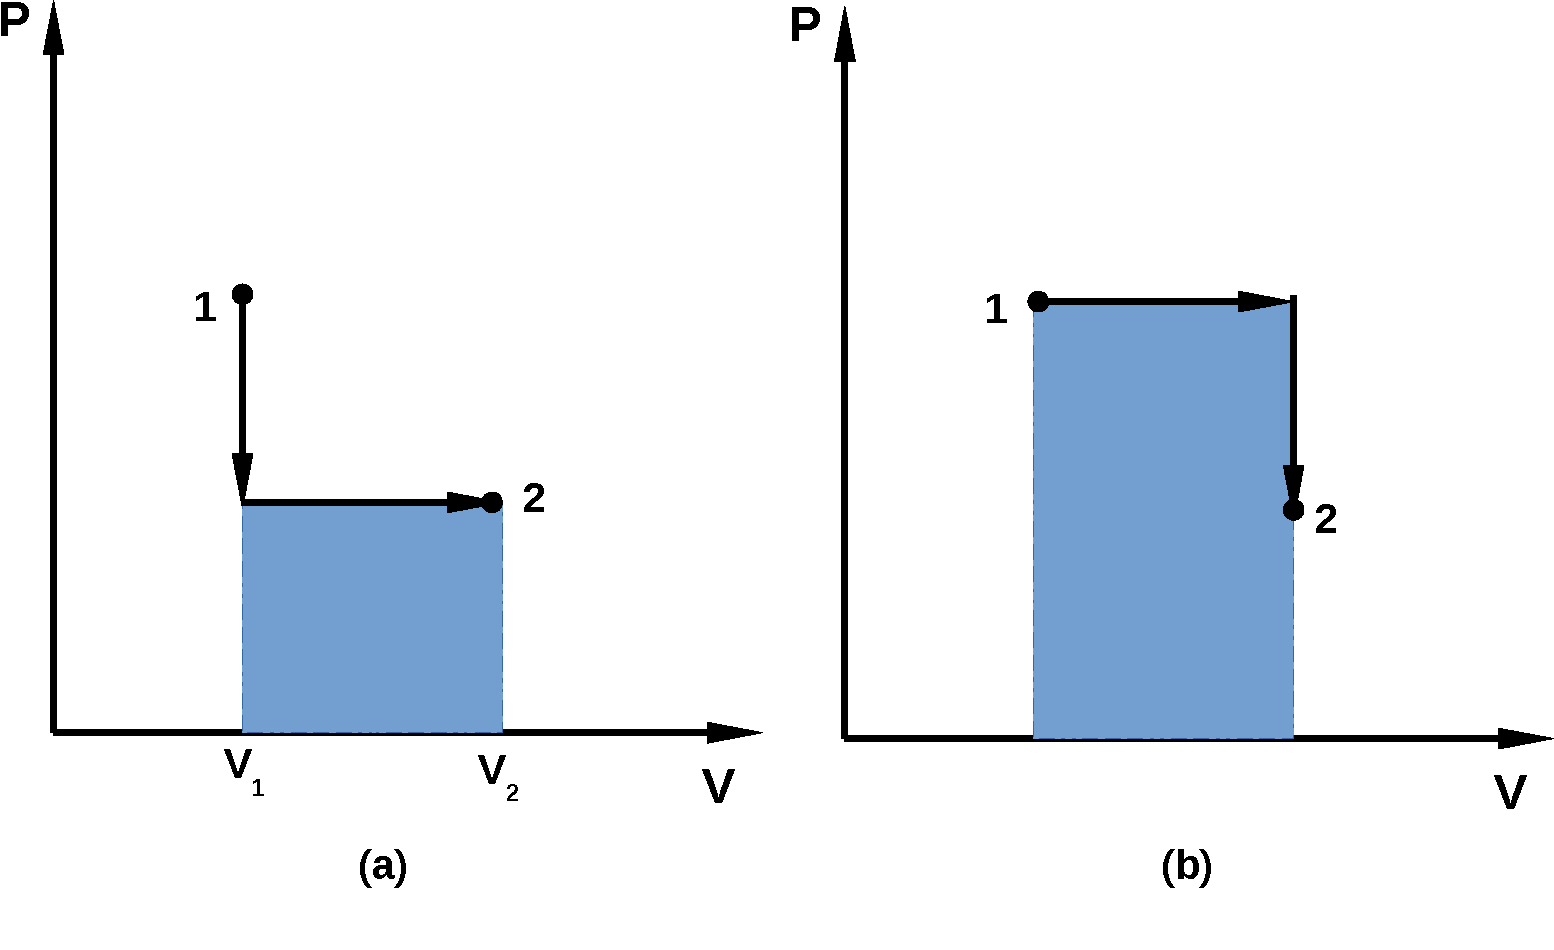
\includegraphics[width=.6\columnwidth,clip]{./Figs/Mod1Ex1}
           \vspace{-.1cm}\caption{Expansion processes (Example~\ref{Mod01Ex01}).}\label{Mod01Fig01}
         \end{center}
       \end{figure}

% SOLUTION
       \noindent{\bf Solution:} $W_{\text{rev}}$ is related to the area below the curve. Thus, we should use the $PV$ work equation:
           \begin{itemize}
              \item For process {\bf (a)}: 
                 \begin{eqnarray}
                    d W = -PdV \Longrightarrow W &=& -P_{2}\left(V_{2}-V_{1}\right) \nonumber \\
                                                 &=& - 1\text{ atm}\left(2000-500\right)\text{ cm}^{3} = -1500\text{ atm.cm}^{3} \nonumber 
                 \end{eqnarray}
                 Now we need to convert {\it atm.cm}$^{3}$ to $J$, thus using the unit conversion table:
                 \begin{eqnarray}
                     W &=& -1500\blue{\cancel{\text{ atm}}}.\red{\cancel{\text{cm}^{3}}} \frc{1.01325\times 10^{5}\blue{\cancel{\text{ Pa}}}}{1\blue{\cancel{\text{ atm}}}} \frc{1 \frc{\text{kg}}{\text{m.s}^{2}}}{1\blue{\cancel{\text{ Pa}}}} \frc{1\text{ m}^{3}}{ 100^{3} \red{\cancel{\text{ cm}^{3}}}} \nonumber \\
                       &=& -151.9875 \blue{\cancel{\frc{\text{ kg.m}^{2}}{\text{s}^{2}}}} \frc{ 1 \text{ J}}{ \blue{\cancel{\frc{\text{ kg.m}^{2}}{\text{s}^{2}}}}} \nonumber\\
                       &=& -151.9875\text{ J} \nonumber
                 \end{eqnarray}
%
              \item For process {\bf (b)}, since $P$ is constant, i.e., $P_{1}=P_{2}$:
                 \begin{eqnarray}
                    d W = -PdV \Longrightarrow W &=& -P_{1}\left(V_{2}-V_{1}\right) \nonumber \\
                                                 &=& - 3\text{ atm}\left(2000-500\right)\text{ cm}^{3} = -4500\text{ atm.cm}^{3} \nonumber \\
                                                 &=& -455.9625\text{ J} \nonumber
                 \end{eqnarray}
           \end{itemize}

\clearpage

%%%
%%% EXAMPLE
%%%
   \item Calculate the internal energy (in $J$) when 1 mol of water is isobarically heated from 25$^{\circ}$C to 30$^{\circ}$C at 1 atm. Given: densities of water are 0.9970 g.cm$^{-3}$ at 0$^{\circ}$C and 0.9956 g.cm$^{-3}$ at 100$^{\circ}$C. Molar mass and heat capacity at constant pressure of water are 18 g.mol$^{-1}$ and 1 cal.$\left(\text{g.}^{\circ}\text{C}\right)^{-1}$, respectively.

% SOLUTION
       \noindent{\bf Solution:} From the 1$^{\text{st}}$ Law, $U=Q+W$ ,and in order to calculate $U$ we first need to obtain heat ($Q$) and work ($W$). $Q$ can be obtained from the heat capacity equation
          \begin{displaymath}
             Q = m C_{p} \Delta T,
          \end{displaymath}  
          where $m$ is the mass of water can be obtained from
          \begin{displaymath}
             n = \frc{m}{MW} \Longrightarrow  m = n.MW = 1\text{ mol} . 18 \frc{\text{g}}{\text{mol}} = 18 \text{ g}
          \end{displaymath}
          $n$ and $MW$ are number of moles and molar mass, respectively. Now,
          \begin{displaymath}
             Q = m C_{p} \Delta T = 18\text{ g} . 1 \frc{\text{ cal}}{\text{g.}^{\circ}\text{C}}.\left(30-25\right)^{\circ}\text{C} = 90\text{ cal}
          \end{displaymath}  
          Now, we should calculate the work through $W=-P\Delta V$, however $V$ is not known, but we can obtain it from the density relation $V=m/\rho$, thus
          \begin{displaymath}
             W = - P\Delta V = -P\left(V_{2}-V_{1}\right) = -P\left(\frc{m}{\rho_{2}} - \frc{m}{\rho_{1}}\right) = -0.025\text{atm.cm}^{3} = -0.0006\text{ cal} 
          \end{displaymath}
          Now, calculating the internal energy,
          \begin{displaymath}
             U = Q + W = 89.9994\cancel{\text{ cal}} . \frc{ 4.186\text{ J}}{1\cancel{\text{ cal}}} = 376.7375 \text{ J}
          \end{displaymath}

\clearpage
%%%
%%% EXAMPLE
%%%
   \item A 0.3 m$^{3}$  tank contains oxygen initially at 100 kPa and 300 K. A paddle wheel within the tank is rotated until the pressure inside rise to 150 kPa. During the process 2 kJ of heat is lost to the surroundings. Determine the paddle-wheel work done (in kJ). Neglect the energy stored in the paddle wheel and assume the heat capacity at constant volume of oxygen is 0.6745 kJ.$\left(\text{kg.K}\right)^{1}$. Given molar mass of oxygen of 32 g.mol$^{-1}$.

% SOLUTION
       \noindent{\bf Solution:} The volume of the tank remains constant $V_{2}=V_{1}=V=$ 0.3 m$^{3}$ during the whole process. Thus, we can define:
            \begin{center}
              \begin{tabular}{l l l l}
                 Initial Condition & $P_{1}=$ 100 kPa   & $T_{1}=$ 300 K         & $V_{1}=$ 0.3 m$^{3}$  \\
                 Final Condition   & $P_{2}=$ 150 kPa   &                       & $V_{2}=$ 0.3 m$^{3}$ \\
                 Heat Loss         & $Q=$ -2 kJ        &                       &                    
              \end{tabular}
            \end{center}
       The compression occurs in a closed system (i.e., constant mass) and, as there is no further information, we may consider that oxygen behaves as an ideal gas. The work added to the system by the paddle can be expressed by $U=Q+W$. Our first step is to calculate $T_{2}$,
       \begin{displaymath}
          \frc{P V}{T} = \text{ constant} \Rightarrow \frc{P_{1}V_{1}}{T_{1}} = \frc{P_{2}V_{2}}{T_{2}} \Rightarrow \frc{P_{1}}{T_{1}}=\frc{P_{2}}{T_{2}} \Rightarrow T_{2} = 450\text{ K}
       \end{displaymath}
        The specific internal energy can defined by the fundamental relation, $du=C_{v}dT$ (check the units for this relation!), where $C_{v}$ is the heat capacity at constant volume thus,
       \begin{displaymath}
          \Delta U = m\Delta u = C_{v}\Delta T = Q + W,
       \end{displaymath}
       therefore, we need to obtain the mass of oxygen in the tank through the ideal gas equation of state,
       \begin{eqnarray}
         P V = n R T \Rightarrow n = \frc{m}{MW} = \frc{P V}{R T} \Rightarrow m &=& \frc{ MW P V}{R T} \nonumber \\
                                                      &=& \frc{ 32\frc{\text{ g}}{\text{mol}} 100\text{ kPa} . 0.3\text{ m}^{3}}{ 8.3143 \frc{\text{J}}{\text{mol.K}} 300\text{ K}} \nonumber \\
                                                      &=& 0.3848 \frc{\text{ g.kPa.m}^{3}}{\text{J}} \frc{1 \text{ J}}{1\text{ N.m}} \frc{1000 \text{ Pa}}{1 \text{ kPa}} \frc{ 1 \text{ N.m}^{-2}}{1\text{ Pa}} \nonumber\\
                                                      &=& 0.3848\text{ kg}\nonumber
       \end{eqnarray}
       Thus
       \begin{eqnarray}
          \Delta u = m C_{v}\Delta T = Q + W \Rightarrow W &=& m C_{v}\left(T_{2}-T_{1}\right) - Q \nonumber \\
                                                          &=& 0.3848\text{ kg} \times 0.6745 \frc{\text{kJ}}{\text{kg.K}}\times (450-300)\text{ K} - (-2 \text{ kJ}) \nonumber \\
                                                          &=& 40.9321\text{ kJ}. \nonumber
       \end{eqnarray}
       The paddle-wheel executed 40.9321 kJ of work to the system.

\clearpage
%%%
%%% EXAMPLE
%%%
   \item  Air initially occupying 1 m$^{3}$ at 1.5 bar and 20$^{\circ}$C undergoes an internally reversible compression for which $P V^{\gamma}=$ constant to a final state where the pressure is 6 bar and the temperature is 120$^{\circ}$C. Determine:
        \begin{enumerate}[(a)]
           \item Value of $\gamma$;
           \item Work and the heat transfer (in kJ).
       \end{enumerate}
       Assume that heat capacity at constant volume and molar mass of air are 0.718 kJ.$\left(\text{kg.K}\right)^{-1}$ and 29 g.mol$^{-1}$. 

% SOLUTION
       \noindent{\bf Solution:}
        \begin{center}
           \begin{tabular}{c c c c}
               {\bf State}  &   $P$ (atm)  &   $T\;\left(^{\circ}\text{C}\right)$ & $V\;\left(\text{m}^{3}\right)$ \\
                    1       &     1.5      &            20                      & 1  \\
                    2       &     6.0      &            120                     &     \\              
           \end{tabular}
        \end{center}
        \begin{enumerate}[(a)]
           \item In order to calculate the isentropic index $\gamma$, we can use any of the relations learned in the lecture,
               \begin{displaymath} 
                   P V^{\gamma} = C, \hspace{1cm} T V^{\gamma-1} = C \hspace{1cm} \text{ and/or } \hspace{1cm} T P^{\frac{1-\gamma}{\gamma}} = C.
               \end{displaymath}
               Although $P$ and $V$ is the relation initially given in the problem, we do not know the final volume of air, $V_{2}$. However, initial and final pressure and temperature are known and we can make use of this relationship to obtain $\gamma$,
               \begin{eqnarray} 
                   T P^{\frac{1-\gamma}{\gamma}} = C \Rightarrow T_{1}P_{1}^{\frac{1-\gamma}{\gamma}} = T_{2}P_{2}^{\frac{1-\gamma}{\gamma}} \nonumber \\
                   \left(\frc{P_{1}}{P_{2}}\right)^{\frac{1-\gamma}{\gamma}} = \frc{T_{2}}{T_{1}} \Rightarrow \frc{1-\gamma}{\gamma} = \frc{\ln{\frac{T_{2}}{T_{1}}}}{\ln{\frac{P_{1}}{P_{2}}}} \Longrightarrow \gamma = 1.2686  \nonumber
               \end{eqnarray}
                 
           \item Compression work can be obtained by integrating $\d W = -P dV$ from state 1 to state 2 with $P=\frac{C}{V^{\gamma}}$,
               \begin{eqnarray}
                 W_{1-2} &=& -\int\limits_{V_{1}}^{V_{2}} P dV = -\int\limits_{V_{1}}^{V_{2}}\frc{C}{V^{\gamma}} dV = -\left.\frc{C}{1-\gamma}V^{1-\gamma}\right|_{V_{1}}^{V_{2}} \nonumber \\
                         &=& -\frc{C}{1-\gamma}\left(V_{2}^{1-\gamma}-V_{1}^{1-\gamma}\right),\;\;\text{ however, as } C=P_{1}V_{1}^{\gamma}=P_{2}V_{2}^{\gamma} \nonumber \\
                         &=& -\frc{P_{2}V_{2}^{\gamma}V_{2}^{1-\gamma} - P_{1}V_{1}^{\gamma}V_{1}^{1-\gamma}}{1-\gamma} = \frc{P_{1}V_{1}-P_{2}V_{2}}{1-\gamma} \nonumber
               \end{eqnarray}
               The relation above, although important, can not be used as we do not know $V_{2}$, however we can change variables through the ideal gas relation
               \begin{eqnarray}
                  P V = n R T &\Rightarrow& n = \frc{P V}{R T } = \frc{1.5\text{ atm} \times 1\text{ m}^{3}}{ 8.3143 \frc{\text{J}}{\text{mol.K}} 293.15\text{ K}} \frc{1.01325\times 10^{5} \text{ Pa}}{1 \text{ atm}} \frc{ 1 \text{ N.m}^{-2}}{1\text{ Pa}}\frc{1 \text{ J}}{1\text{ N.m}} = 62.3580\text{ moles}\nonumber \\
                   % m &=& \frc{P_{1} V_{1} MW}{R T_{1}} = \frc{1.5\text{ atm} \times 1\text{ m}^{3} \times 29 \frac{\text{g}}{\text{mol}} } { 8.3143 \frc{\text{J}}{\text{mol.K}} 293.15\text{ K}} \frc{1 \text{ J}}{1\text{ N.m}} \frc{1.01325\times 10^{5} \text{ Pa}}{1 \text{ atm}} \frc{ 1 \text{ N.m}^{-2}}{1\text{ Pa}} = 1808.38 \text{ g}\nonumber\\
                    W &=& \frc{P_{1}V_{1}-P_{2}V_{2}}{1-\gamma} = nR\frc{T_{1}- T_{2}}{1-\gamma} \nonumber \\
                      &=& 62.3580\text{ mol} \times 8.3143 \frc{\text{J}}{\text{mol.K}} \times \frc{\left(293.15-393.15\right)\text{ K}}{1-1.2686} \nonumber \\
                      &=& 193024.2440 \text{ J} \Longrightarrow W = -193.02 \text{ kJ} \nonumber
               \end{eqnarray}
              Heat ($Q$) can be obtained from
               \begin{eqnarray}
          \Delta u &=& m C_{v}\Delta T = n MW C_{v}\Delta T = Q + W  \nonumber \\
             Q &=& n MW C_{v}\left(T_{2}-T_{1}\right) - W \nonumber \\
               &=& 62.3580\text{ mol}\times 29 \frc{\text{g}}{\text{mol}} \red{\frc{1\text{ kg}}{1000\text{ g}}}\times 0.718\frc{\text{kJ}}{\text{kg.K}}\times (393.15-293.15)\text{ K} - 193.30 \text{ kJ} \nonumber \\
                                                          &=& -63.46\text{ kJ}. \nonumber                   
               \end{eqnarray}
       \end{enumerate}


\clearpage
%%%
%%% EXAMPLE
%%%
   \item Two kg of water at 80$^{\circ}$C is mixed adiabatically with 3 kg of water at 30$^{\circ}$C in a constant pressure process of 1 atm. Find the increase in entropy $\left(\text{in kJ.K}^{-1}\right)$ of the total mass of water due to the mixing process. Assume that $C_{p}$ of water is 4.187 kJ.$\left(\text{kg.K}\right)^{-1}$. 

% SOLUTION
       \noindent{\bf Solution:} From the classic thermodynamic definition of reversible entropy processes (second law),
         \begin{displaymath}
            d S = \frc{d Q}{T}
         \end{displaymath}
         with $dQ = m C_{p}dT$, then integrating 
         \begin{eqnarray}
            \int\limits_{S_{i}}^{S_{f}} dS &=& m C_{p}\int\limits_{T_{i}}^{T_{f}}\frc{dT}{T} \nonumber \\
            \Delta S &=& S_{f}-S_{i} = m C_{p} \ln{\frc{T_{f}}{T_{i}}} \nonumber
         \end{eqnarray}
         Assuming that the system is adiabatic, we can calculate the final temperature $\left(T_{f}\right)$ from thermal energy conservation principles: 
         \begin{displaymath}
            m_{1}C_{p,1}T_{1} + m_{2}C_{p,2}T_{2} = \left(m_{1}+m_{2}\right)C_{p}T_{f} \rightarrow T_{f} = 50^{\circ}\text{C} = 323.15\text{ K}
         \end{displaymath}
         And the entropies are
         \begin{eqnarray}
             \Delta S_{1} &=& m_{1}C_{p,1}\ln{\frc{T_{f}}{T_{1}}} =  -0.7434\frc{\text{kJ}}{\text{K}} \nonumber \\
             \Delta S_{2} &=& m_{2}C_{p,2}\ln{\frc{T_{f}}{T_{2}}} =  0.8025\frc{\text{kJ}}{\text{K}} \nonumber 
         \end{eqnarray}
         Thus the increase in entropy of the total mass is
         \begin{displaymath}
              \Delta S_{\text{mix}} = \Delta S_{1} + \Delta S_{2} = 0.0591\frc{\text{kJ}}{\text{K}}
         \end{displaymath}
%
\end{enumerate}

\clearpage
%%%%%%%%%%%%%%%%%%%%%%%%%%%%%%%%%%%%%%%%%%%%%%%%%%%%%%%%%%%%%%%%%%%%%%%%%%%%%%%%%%%%%%%%%%%%%%%%%%%%%%%%%%%%%%%%%%%%%%%%%%%%%%%%%%%%%%%%%%%%%%
%%%%%%%%%%%%%                                                    END OF MODULE 01                                                %%%%%%%%%%%%%
%%%%%%%%%%%%%%%%%%%%%%%%%%%%%%%%%%%%%%%%%%%%%%%%%%%%%%%%%%%%%%%%%%%%%%%%%%%%%%%%%%%%%%%%%%%%%%%%%%%%%%%%%%%%%%%%%%%%%%%%%%%%%%%%%%%%%%%%%%%%%%

%%%
%%% SECTION
%%%
\section{Module 02: Volumetric Properties of Pure Fluids}\label{Section:02}


%%% SUBSECTION
\subsection{PVT Behaviour of Pure Substances}
  
   \begin{enumerate}[i)]
%
       \item {\it Pure substances/fluids} can be defined as a material of homogeneous and constant composition. Systems containing (a) water and ice, (b) water and steam or (c) water, ice and steam are examples of pure fluids at different phases, whereas (d) air-water, (e) air-steam and (f) a gaseous mixture containing N$_{2}$, H$_{2}$, O$_{2}$ and NO$_{2}$ are not. 
%
       \item A pure fluid can exist and coexist in different phases (\ie solid, liquid and vapour -- S, L and V). Phase behaviour of fluids is often represented by {\it PVT}\footnote{{\it PVT} stands for pressure, specific (or molar) volume and temperature.} phase diagrams. 
%
       \item {\it PVT} diagram of an arbitrary fluid is shown as 3D representation in Figure~\ref{Mod02Fig01}a. Solid, liquid and vapour phases are represented by continuous volumes and, the regions between these volumes are representations of \blue{phase equilibrium}.
%
           \begin{figure}[h]
              \begin{center}
                 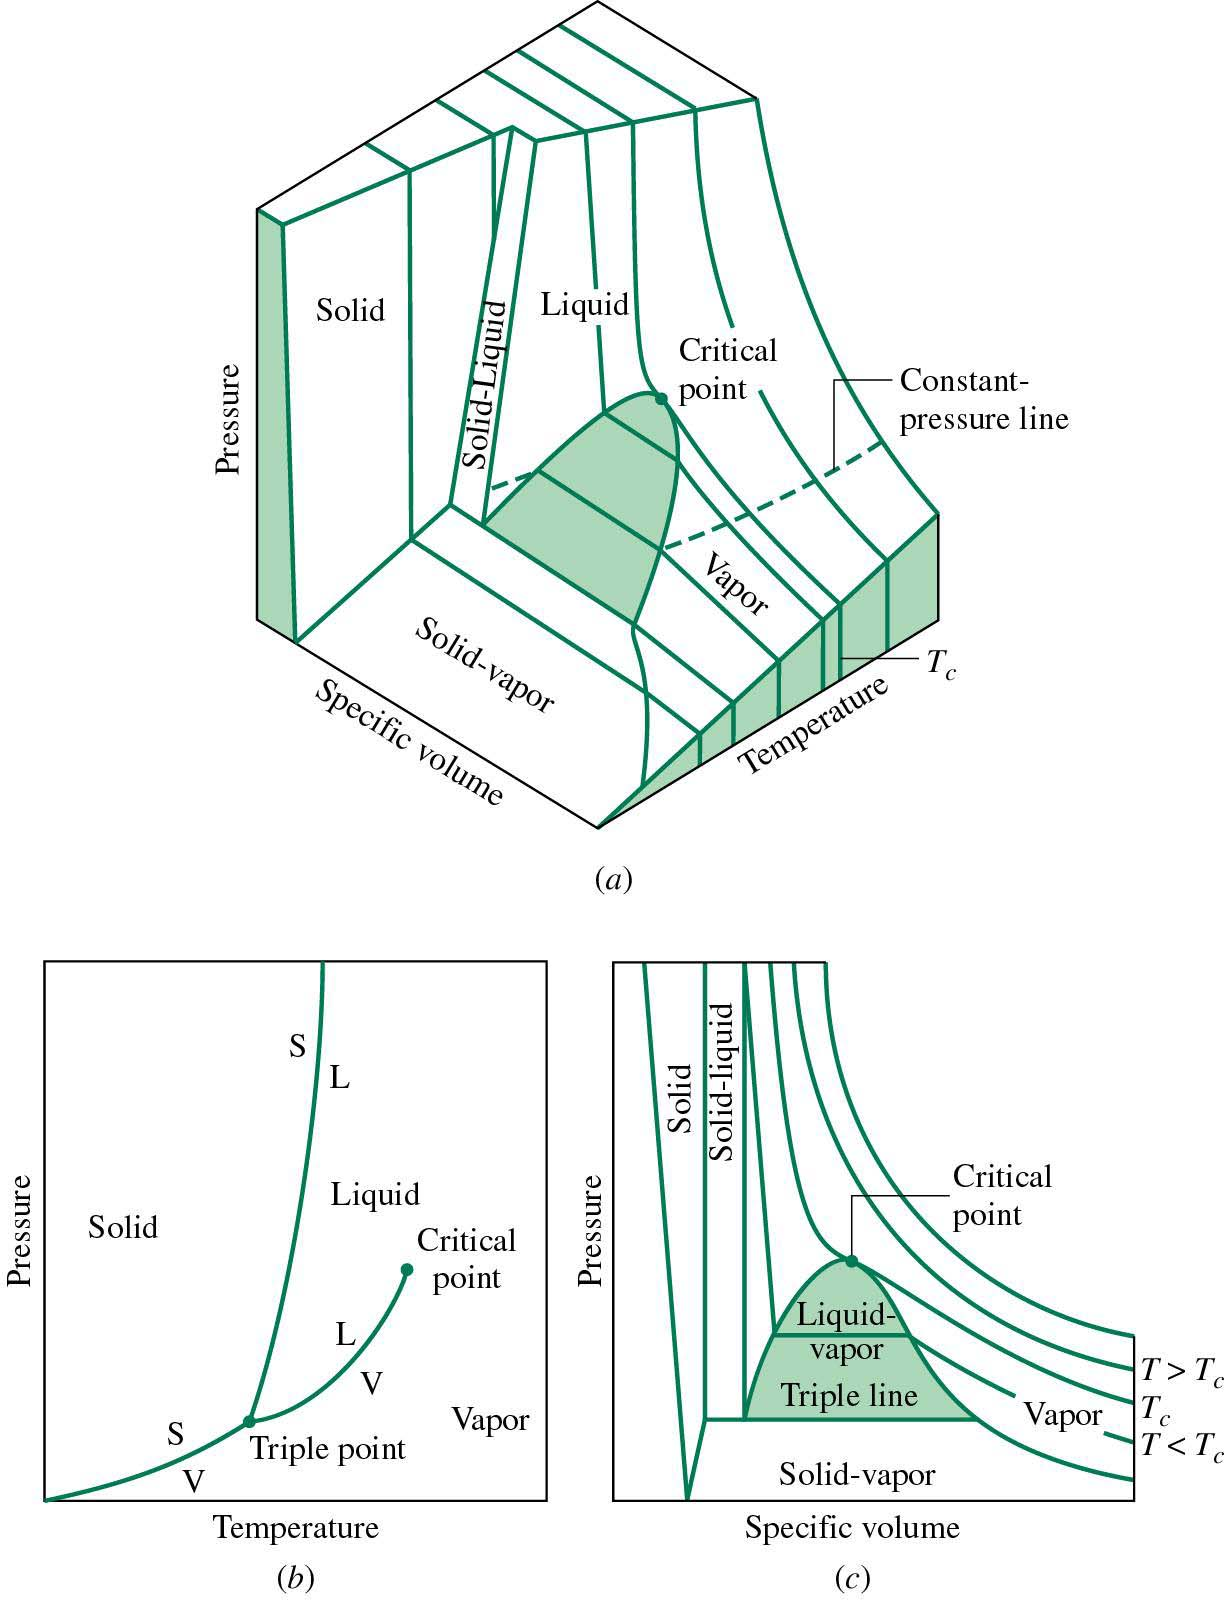
\includegraphics[width=10.cm,clip]{./../Pics/PVT_Surface.jpg}\label{Mod02Fig01}
                 \caption{$PVT$ volume (top) and projections onto (b) $PT$ and (c) $PV$ diagrams for a pure substance (Extracted from Borgnakke $\&$ Sonntag).}\label{Mod02Fig01}
              \end{center}
           \end{figure}    
%
       \item Such 3D representation helps determining (qualitatively) phases (S, L and V) at prescribed coordinates (temperature, specific/molar volume and pressure) of fluids. However, it is not convenient dealing with 3D plots and, most of the time, we may want to extract quantitative values of fluids (Module 03). A better approach is to project 3D plots into surfaces, \ie $PT$, $PV$ and $VT$ diagrams (Figs.~\ref{Mod02Fig01}b and~\ref{Mod02Fig01}c).
%
       \item $PV$ diagrams (Fig.~\ref{Mod02Fig02}a) are representations of Fig.~\ref{Mod02Fig01}a at constant specific temperature, where surfaces represent both single phases and phase transitions (\ie phases in equilibrium). Here, there are three properties that we need to define:
           \begin{enumerate}[a)]
              \item Critical point (or state): coordinates in which two phases of a fluid become indistinguishable. Beyond this coordinate, a fluid is neither completely liquid nor completely gaseous, \ie exhibits properties of both the liquid phase and the gas phase and is referred to as a {\it supercritical fluid}. All fluids have distinct critical coordinates, known as {\it critical pressure} $\left(\text{P}_{c}\right)$, {\it critical temperature} $\left(\text{T}_{c}\right)$ and {\it critical volume} $\left(\text{V}_{c}\right)$. Interesting videos about critical state can be seen in \href{https://www.youtube.com/watch?v=bJjcTpRzXpM}{https://www.youtube.com/watch?v=bJjcTpRzXpM} and \href{https://www.youtube.com/watch?v=RmaJVxafesU}{https://www.youtube.com/watch?v=RmaJVxafesU}.
              \item Saturation lines (blue lines in Fig.~\ref{Mod02Fig02}a) are coordinates in which phase transition starts to occur.
              \item Isotherms: Lines of constant temperature.
           \end{enumerate} 
           In vapour-liquid equilibrium (VLE) systems there are two main saturation lines: {\it saturated liquid line} (left-hand side of $C$ in Fig.~\ref{Mod02Fig02}a)  and {\it saturated vapour line} (rhs of $C$) that represent the initial transition from a single phase system to a two or three phases system. 
%
       \item $PT$ diagrams (Fig.~\ref{Mod02Fig02}b) are representations of Fig.~\ref{Mod02Fig01}a at constant specific volumes, where phases are defined by surfaces with continuous lines representing phases transitions (\ie in equilibrium). The {\it triple point} is coordinate in which all three phases (S, L and V) coexist in equilibrium.
%
           \begin{figure}[h]\label{Mod02Fig02}
              \vbox{
                    \hbox{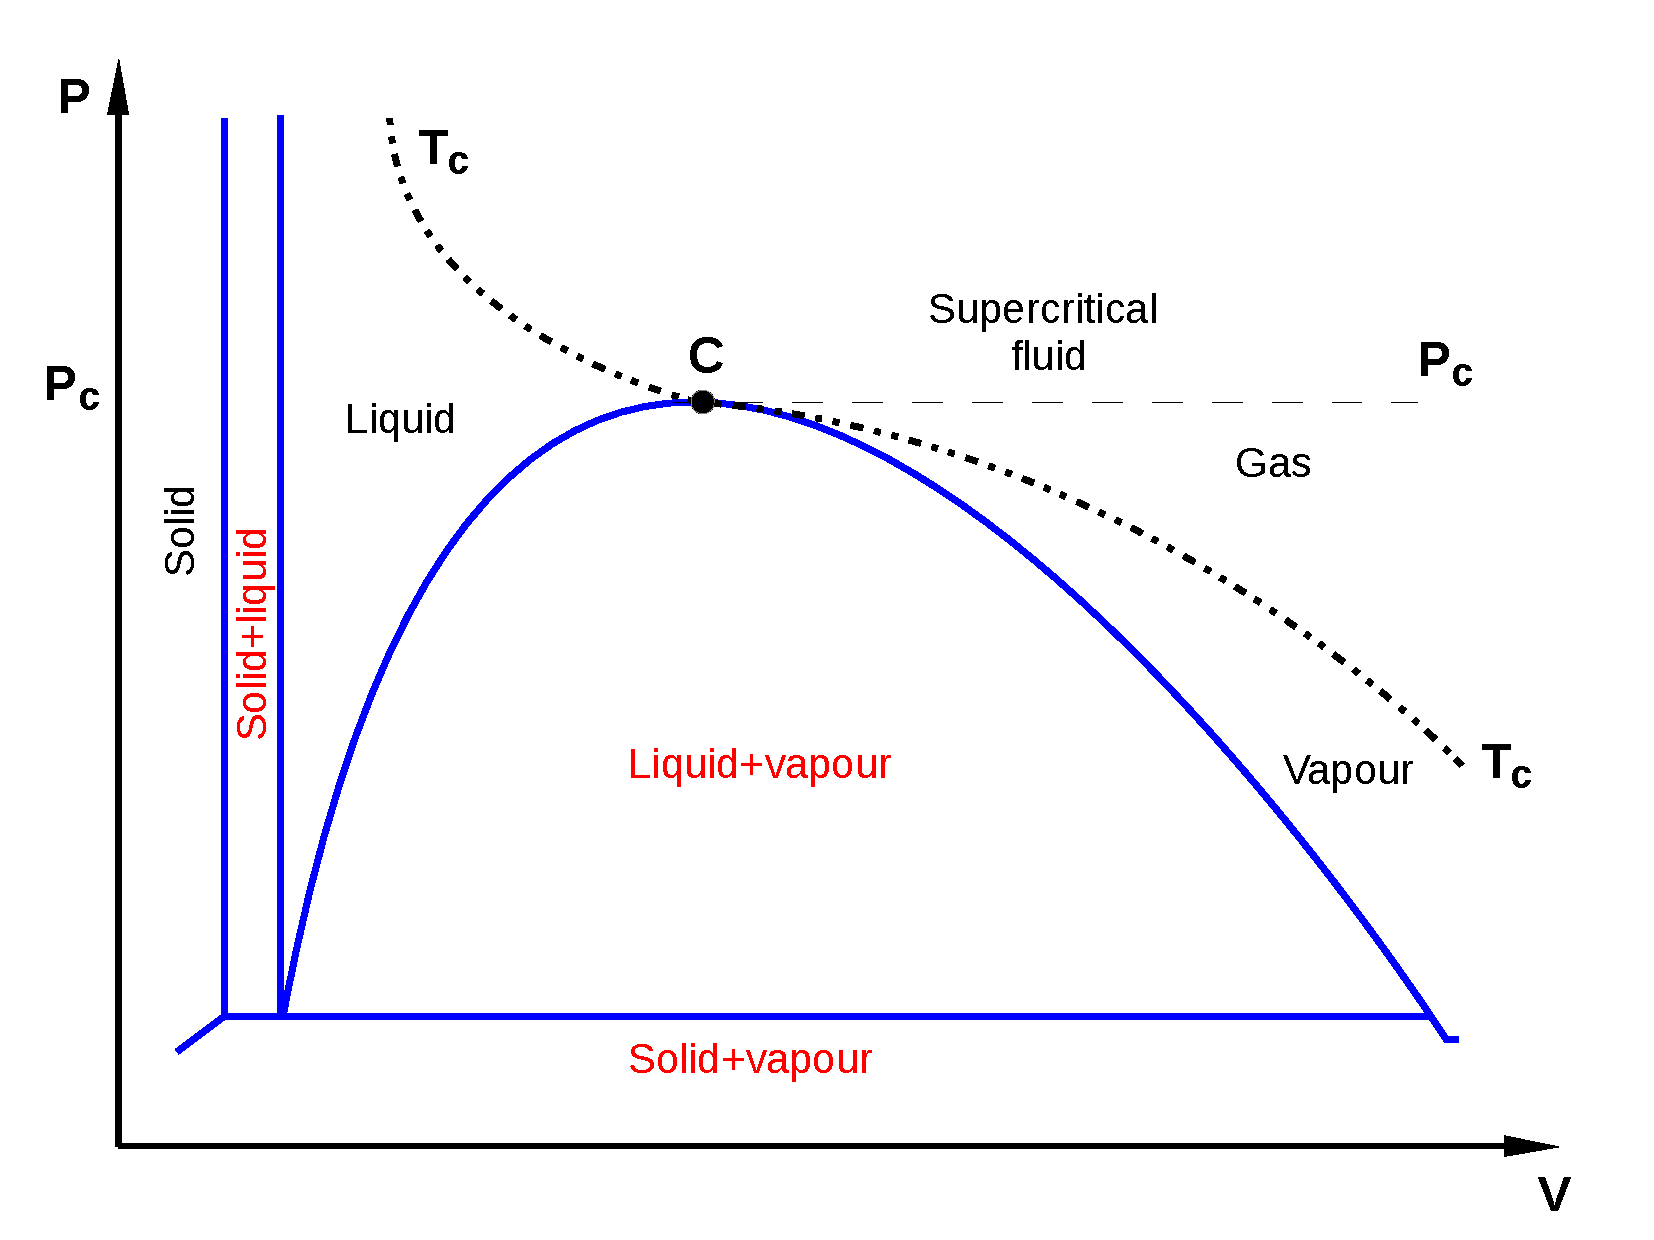
\includegraphics[width=.5\columnwidth,clip]{./../Pics/PV_Diagram1}
                          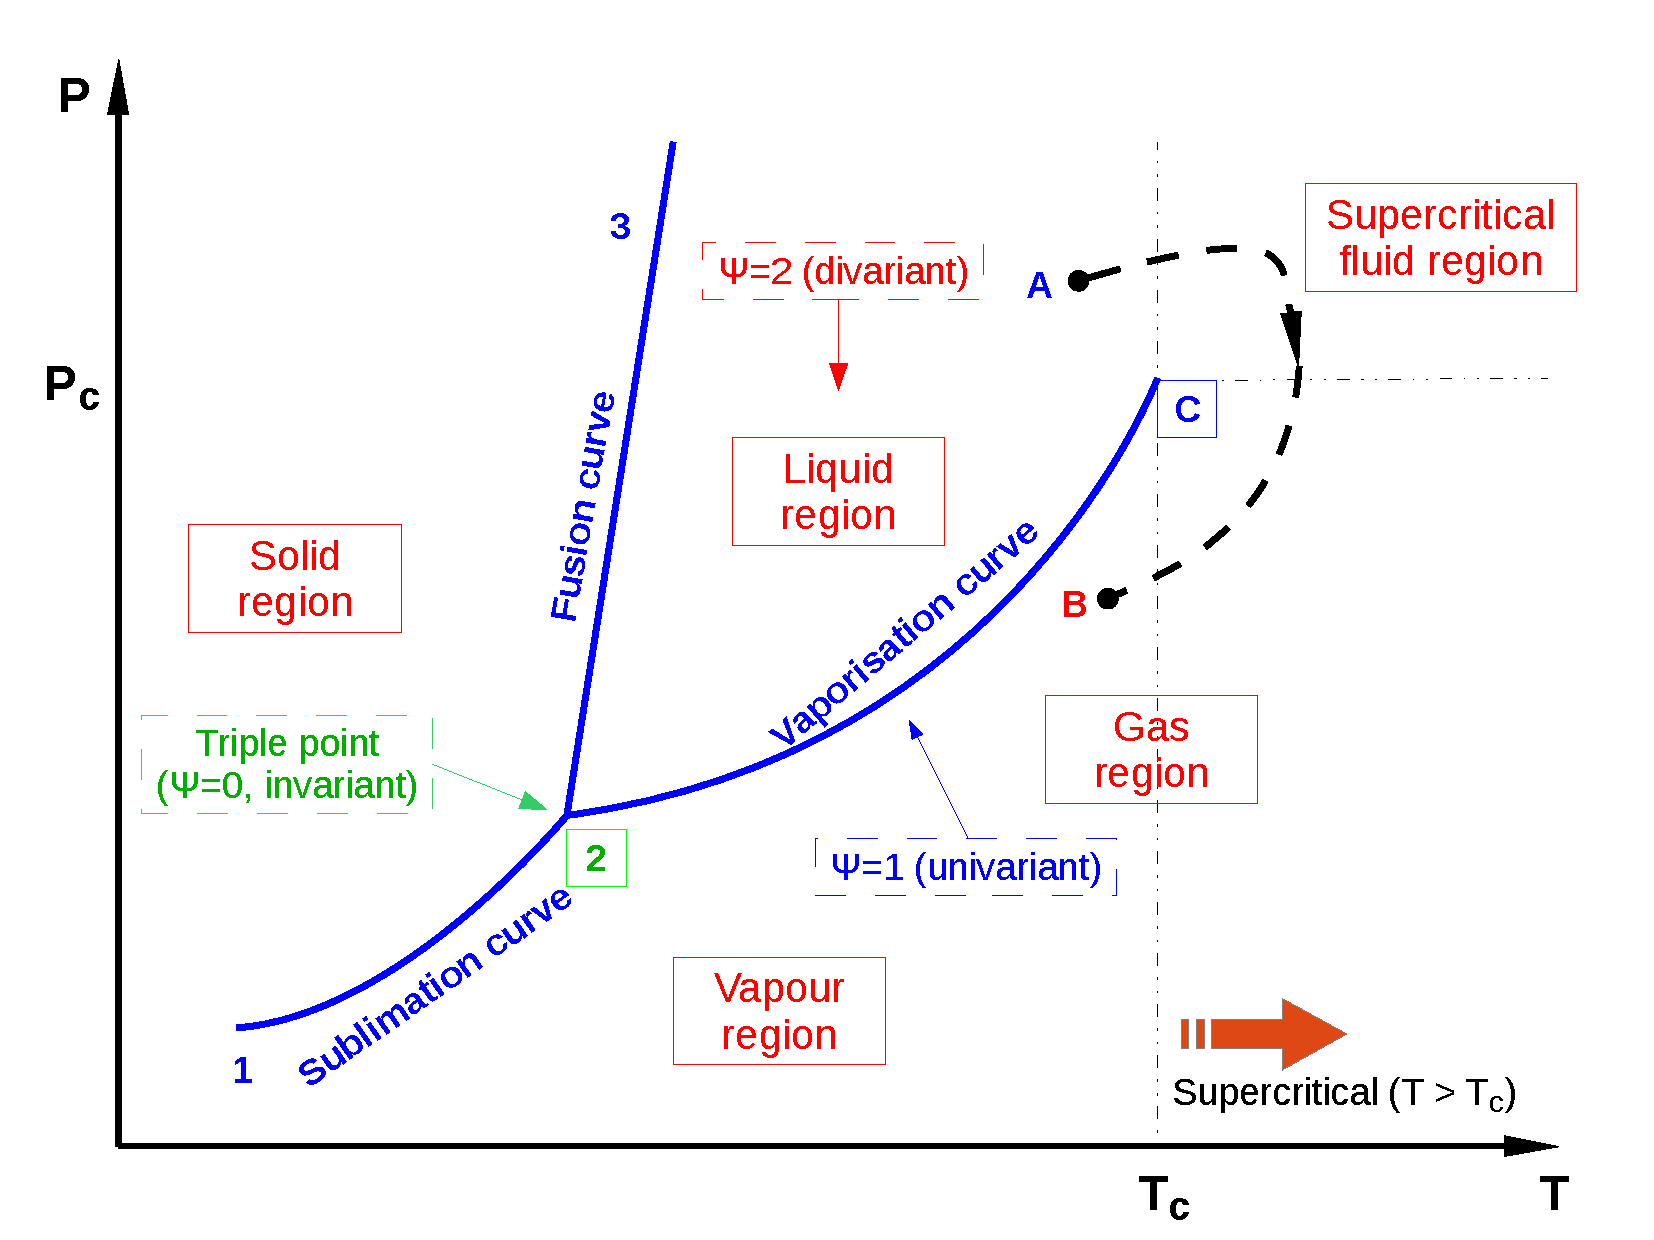
\includegraphics[width=.5\columnwidth,clip]{./../Pics/PT_Diagram}}
                    \vspace{-.1cm}
                    \hbox{\hspace{4cm}(a)\hspace{8cm}(b)}}
              \caption{ (a) $PV$ and (b) $PT$ diagrams for a pure substance. Dotted line in (a) represents the isotherm at T=T$_{c}$.}\label{Mod02Fig02}
           \end{figure}
%
        \item A fluid in the compressed liquid state is often called {\it sub-cooled fluid} (central region of Fig.~\ref{Mod02Fig02}b), while a gas at a pressure lower than its saturation vapour pressure for a given temperature is said to be at {\it superheated state}.
%
        \item The \underline{Gibbs phase rule} is a relation that determines the number of independent variables that mist be specified to establish the {\it intensive state of any system at equilibrium},
                \begin{equation}
                    \Psi = 2 + \mathcal{C} - \mathcal{P} -\mathcal{R},\label{Mod02_GibbsPhaseRuleReactive}
                \end{equation}
                where $\Psi$, $\mathcal{C}$, $\mathcal{P}$ and $\mathcal{R}$ are the number of degrees of freedom of the thermodynamic system, number of chemical components, number of co-existing phases and number of independent reactions, respectively. For non-reactive systems\footnote{The Gibbs phase rule will be revisited again in Module~\ref{Section:06} -- Chemical Reaction Equilibrium.}, this relation becomes,
                \begin{equation}
                    \Psi = 2 + \mathcal{C} - \mathcal{P}.\label{Mod02_GibbsPhaseRule}
                \end{equation}
                The degrees of freedom ($\Psi$, \ie number of intensive properties such as temperature and pressure) determines the number of variables that must be specified to fix all other remaining phase rule variables. For example, for a pure liquid component, the phase rule yields two degrees of freedom, \ie if temperature and pressure are specified, all other intensive properties (\eg enthalpy, entropy etc) are uniquely determined. However, if the same liquid component is in equilibrium with its vapour phase (\eg water and steam) there is {\it only} one degree of freedom. This means that either pressure or temperature may be specified to fix all other intensive properties of the system. At the triple point (\eg water, steam and ice), the number of degrees of freedom is {\it zero}, \ie any change from such state (\eg for water-steam-ice at $\sim$ 273.15 K and 0.0061 bar) causes at least one of the phases to vanish.
%
        \item The ideal gas {\it equation of state} (EOS),
                \begin{equation}
                   P V = R T,\label{Mod02_IdealEOS}
                \end{equation}
                where $V$ is the molar volume. This is a relationship between the macroscopic intensive properties, and is based in two main assumptions with respect to the microscopic behaviour of molecules:
            \begin{enumerate}[(a)]
                \item Molecules have no extension in space (\ie zero volume), and;
                \item Molecules \underline{do not interact with each other}.
            \end{enumerate}
            The second assumption is particularly important as it considers that atoms and molecules either do not interact or do not have electric charge or have an infinite distance between them (\ie at low density conditions).
%
        \item However, these assumptions are rarely met in real conditions (both in the environment and in industry) and several mathematical relations have been developed to better represent the PVT behaviour of real fluids:
            \begin{enumerate}[a)]
%
                \item The PVT behaviour of real pure fluids can be expressed as functional $f(P,V,T) = 0$. However, from the Gibbs phase rule for a single phase pure component the number of degrees of freedom is equal to 2. Therefore, we can write this function in its simplest way (or EOS), $V=V(T,P)$, or in differential form,
                   \begin{displaymath}
                      dV = \left(\frc{\partial V}{\partial T}\right)_{P}dT + \left(\frc{\partial V}{\partial P}\right)_{T}dP
                   \end{displaymath}
                   defining the {\it coefficient of thermal expansion} (or {\it volume expansivity coefficient}), $\beta$, and the {\it coefficient of isothermal compressibility}, $\kappa$ as,
                   \begin{equation}
                      \beta \equiv \frc{1}{V}\left(\frc{\partial V}{\partial T}\right)_{P}\;\;\;\text{ and }\;\;\;\kappa \equiv -\frc{1}{V}\left(\frc{\partial V}{\partial P}\right)_{T},\label{Mod02_Compressibilityexpansivity}
                   \end{equation}
                   respectively, leading to
                   \begin{equation}
                       \frc{dV}{V} = \beta dT - \kappa dP.\label{Mod02_Compressibilityexpansivity2}
                   \end{equation}
%
                \item The {\it Virial EOS} is a relation that can be derived from statistical mechanics, and is represented by power series in terms of $\frac{1}{V}$ with two alternate forms:
                   \begin{eqnarray}
                       \frc{P V}{R T} &=& 1 + \frc{B}{V} + \frc{C}{V^{2}} + \cdots \text{ or} \label{Mod02_Virial1}\\
                       \frc{P V}{R T} &=& 1 + B^{\prime}P + C^{\prime}P^{2} + \cdots,\label{Mod02_Virial2} 
                   \end{eqnarray}
                   where $B$ and $C$ are the second and third virial coefficients and,
                   \begin{displaymath}
                      B = \frc{B^{\prime}}{R T}\;\;\;\text{ and }\;\;\; C^{\prime}=\frc{C-B^{2}}{\left(R T\right)^{2}}.
                   \end{displaymath}
                   Second and third terms of Eqns.~\ref{Mod02_Virial1} and~\ref{Mod02_Virial2} are \blue{corrections of the non-ideal behaviour of a gas}. Virial coefficients are strongly dependent on the temperature (\ie $B=B(T)$, $C=C(T)$, $D=D(T)$ etc) and the more the number of coefficients (\ie the more terms in the power series -- Eqns.~\ref{Mod02_Virial1} and~\ref{Mod02_Virial2}) the better is the predictions of the gas molar volume. The second virial coefficient is readily found for a large number of fluids in any chemical engineering handbook (and several textbooks), however the third and further coefficients are more difficult to obtain/calculate. Therefore the Virial EOS is often used for moderate deviations from the ideal gas behaviour through the truncated forms of Eqns.~\ref{Mod02_Virial1} and~\ref{Mod02_Virial2}
                   \begin{eqnarray}
                      \frc{P V}{R T} &=& 1 + \frc{B}{V} \;\;\;\;\text{ or } \label{Mod02_Virial1b}\\
                      Z &=& 1 + \frc{B P}{R T} = 1 + \frc{B P_{c}}{R T_{c}}\frc{P_{r}}{T_{r}},\label{Mod02_Virial1c}
                   \end{eqnarray}
                   where,
                   \begin{equation}
                      T_{r} = \frc{T}{T_{c}}\;\;\;\;\text{ and }\;\;\;\; P_{r} = \frc{P}{P_{c}}\label{Mod02_ReducedT-P},
                   \end{equation}
                   are {\it reduced temperature and pressure}, respectively. $Z = \frac{P V}{R T}$ is the \underline{compressibility factor} and can be defined as the ration of the molar volume of a gas to the molar volume of an ideal gas at the same temperature and pressure conditions -- for an ideal gas, $Z=1$. 

                   A number of {\it generalised relations} have been developed to calculate the {\it second virial coefficients}, \eg
                   \begin{displaymath}
                      \frc{B P_{c}}{R T_{c}} = B^{0} + \omega B^{1},
                   \end{displaymath}
                   with terms $B^{0}$ and $B^{1}$ defined by,
                   \begin{displaymath}
                      B^{0} = 0.083 - \frc{0.422}{T_{r}^{1.6}}\;\;\text{ and }\;\; B^{1} = 0.139 - \frc{0.172}{T_{r}^{4.2}}.
                   \end{displaymath}
                   $\omega$ is a parameter known as \underline{acentric factor} that measures the non-sphericity of molecules,
                   \begin{displaymath}
                      \omega \equiv -1 - \log\limits_{10}{\left(P_{r}^{\text{sat}}\right)_{T_{r}=0.7}},
                   \end{displaymath}
                   where $\left(P_{r}^{\text{sat}}\right)_{T_{r}=0.7}$ is the reduced saturation vapour pressure obtained at reduced temperature of 0.7. 
%
                \item The truncated form of the {\it Virial EOS} can be used to represent PVT behaviour of gases with reasonable accuracy at relatively low pressures. At moderate and high pressures, predicted volumetric properties deviate from expected and alternative EOS formulations have been developed. \underline{Cubic EOS} are widely used in flow and process simulators to represent PVT behaviour of fluids, and were developed as a cubic function of the molar volume (or the compressibility factor, $Z$). Cubic equations of state can result in (reasonable) accurate prediction of both gas and liquid (saturated) molar volumes and are relatively easy to implement. Since the development of the first cubic EOS in the 19$^{\text{th}}$ century, several EOS have been proposed and used by industry. Four of the most important cubic EOS are listed below:
                   \begin{enumerate}[c.1)]
%
                      \item The \underline{van der Walls} (vdW) EOS was originally developed in 1873 and has the form,
                          \begin{equation}
                             P = \frc{R T}{V-b} - \frc{a}{V^{2}},\label{Mod02_vdWEOS}
                          \end{equation}
                          where $a$ is called the {\it attraction parameter} and $b$ is the {\it repulsive parameter} (or {\it effective molecular volume} or {\it co-volume}), 
                          \begin{displaymath}
                              a = \frc{27}{64}\frc{R^{2}T_{c}^{2}}{P_{c}},\;\;\; b = \frc{1}{8}\frc{R T_{c}}{P_{c}},
                          \end{displaymath}
                          and they take into account interactions between molecules. Although this EOS is able to predict volumetric properties of gasses better than the ideal EOS, it is still very inaccurate for liquids and for fluids at high pressure.  Redlich-Kwong and Soave-Redlich-Kwong were formulated in the 40's and 70's and became increasingly popular in the oil $\&$ gas and petrochemical sectors. 
%
                      \item Redlich-Kwong (RK EOS):
                           \begin{equation}
                               P = \frc{R T}{V-b} - \frc{a}{V\sqrt{T}\left(V+b\right)},\label{Mod02_RKEOS}
                           \end{equation}
                           with,
                          \begin{displaymath}
                              a = \frc{0.42748 R^{2}T_{c}^{2}}{P_{c}},\; \text{ and }\;\;\; b = \frc{0.08664 R T_{c} }{P_{c}}.
                          \end{displaymath}
%
                      \item Soave-Redlich-Kwong (SRK EOS):
                           \begin{equation}
                               P = \frc{R T}{V-b} - \frc{a\alpha}{V\left(V+b\right)},\label{Mod02_SRKEOS}
                           \end{equation}
                           with,
                          \begin{eqnarray}
                              &&a = \frc{0.427 R^{2}T_{c}^{2}}{P_{c}},\;\;\;b = \frc{0.08664 R T_{c} }{P_{c}} \nonumber \\
                              &&\text{and }\;\;\; \alpha = \left[1 + \left( 0.48508 + 1.55171\omega - 0.15613\omega^{2}\right)\left(1-\sqrt{T_{r}}\right)\right]^{2}\nonumber
                          \end{eqnarray}                          
%
                      \item Peng-Robinson (PR EOS):
                           \begin{equation}
                               P = \frc{R T}{V-b} - \frc{a\alpha}{V\left(V+b\right)+b\left(V-b\right)},\label{Mod02_PREOS}
                           \end{equation}
                           with,
                          \begin{eqnarray}
                              && a = \frc{0.45274 R^{2}T_{c}^{2}}{P_{c}},\;\;\;b = \frc{0.07780 R T_{c} }{P_{c}},\;\;\alpha = \left[1 + \kappa\left(1-\sqrt{T_{r}}\right)\right]^{2}  \nonumber \\
                              &&\text{ and }\; \kappa = 0.37464 + 1.54226\omega - 0.26992\omega^{2} \nonumber
                          \end{eqnarray}                
%
                   \end{enumerate}
                   These EOS can be generalised and manipulated to appear as a cubic function of the compressibility factor, $Z$,
                   \begin{equation}
                      Z^{3} + k_{1} Z^{2} +k_{2} Z + k_{3} = 0,\label{Mod02_GeneralEOS}
                   \end{equation}
                   where
                   \begin{eqnarray}
                     && A = \frc{aP}{\left(RT\right)^{2}},\;\; B = \frc{bP}{RT},\;\; k_{1} = -1 -B + uB, \nonumber \\
                     && k_{2} = A + w B^{2} - uB -uB^{2}\;\;\text{ and }\;\; k_{3} = - AB -w B^{2} -w B^{3}.\nonumber
                   \end{eqnarray}

\begin{table}[h]
  \begin{center}
  \begin{tabular}{ c | c c c c c }
    \hline
      {\bf EOS} & {\bf $u$} & {\bf $w$} & {\bf k$_{1}$} & {\bf k$_{2}$} & {\bf k$_{3}$} \\
    \hline
        {\bf vdW} &    0    &    0    & -1-B       &     A         & -AB         \\
        {\bf RK}  &    1    &    0    & -1         &  A-B-B$^{2}$   & -AB         \\
        {\bf SRK} &    1    &    0    & -1         &  A-B-B$^{2}$   & -AB         \\
        {\bf PR}  &    2    &   -1    & -1+B       & A-2B-3B$^{2}$  & -AB+B$^{2}$+B$^{3}$ \\
    \hline
  \end{tabular}
  \caption{Values for $u$, $w$ and k$_{i}$ for vdW, RK, SRK and PR EOS --  Eqn.~\ref{Mod02_GeneralEOS}.}\label{Mod02:Table1}
  \end{center}
\end{table}
                   Coefficients for these expressions are listed in Table~\ref{Mod02:Table1}. Equation~\ref{Mod02_GeneralEOS} has three roots ($Z_{1}$, $Z_{2}$ and $Z_{3}$), the largest \underline{real positive root} represents the {\it vapour phase}, $Z_{\text{vap}}$, whereas the \underline{smallest real positive root} represents the {\it liquid phase}, $Z_{\text{liq}}$. Intermediate root has no physical meaning. The relevant roots for this cubic polynomial can be solved through:
                   \begin{eqnarray}
                       Z_{\text{vap}} = 1 + \beta - q\beta \frc{Z - \beta} {\left(Z+\varepsilon\beta\right)\left(Z+\sigma\beta\right)},\label{Mod02_Zvap} \\
                       Z_{\text{liq}} = 1 + \beta + \left(Z + \epsilon\beta\right)\left(Z+\sigma\beta\right)\left(\frc{1+\beta-Z}{q\beta}\right)\label{Mod02_Zliq}
                   \end{eqnarray}
                   with 
                   \begin{displaymath}
                      \beta=\Omega\frc{P_{r}}{T_{r}},\;\;\; \text{ and }\;\;\; q=\frc{\Psi\alpha}{\Omega T_{r}}.
                   \end{displaymath}
                   Parameters for these expressions are listed in Table~\ref{Mod02:Table2} with
                   \begin{eqnarray}
                         \alpha_{\text{SRK}} &=& \left[ 1 + \left( 0.480 + 1.574 \omega - 0.176\omega^{2}\right)\left(1-\sqrt{T_{r}}\right)\right]^{2}, \nonumber \\
                         \alpha_{\text{PR}} &=& \left[ 1 + \left( 0.37464 + 1.54226 \omega - 0.26992\omega^{2}\right)\left(1-\sqrt{T_{r}}\right)\right]^{2}. \nonumber
                   \end{eqnarray}
                   Equations~\ref{Mod02_Zvap} and ~\ref{Mod02_Zliq} can be numerically solved either using a {\it calculator} or applying any method described in Appendix \red{E.2}.


\begin{table}[h]
    \begin{center}
       \begin{tabular}{| l | c c c c c| }
       \hline
          {\bf EOS}  & {\bf $\alpha$} & {\bf $\sigma$}  & {\bf $\varepsilon$} & {\bf $\Omega$} & {\bf $\Psi$ } \\
       \hline
            vdW      & 1              & 0               & 0                  & 1/8            & 27/64          \\
            RK       & T$_{r}^{-1/2}$  & 1                & 0                  & 0.08664       & 0.42748        \\
           SRK       &$\alpha_{\text{SRK}}$& 1            & 0                   & 0.08664       & 0.42748        \\
            PR       &$\alpha_{\text{PR}}$& 1+$\sqrt{2}$   & 1-$\sqrt{2}$        & 0.07780        & 0.45724  \\
       \hline
       \end{tabular}
  \caption{Parameters for Eqns.~\ref{Mod02_Zvap}-~\ref{Mod02_Zliq}.}\label{Mod02:Table2}
  \end{center}
\end{table}

                  

%
            \end{enumerate}
% 
   \end{enumerate}

\clearpage

%%% SUBSECTION
\subsection{Examples}

\begin{enumerate}[1)]
%%%
%%% EXAMPLE 
%%%
\item\label{Mod02Ex01} For gaseous methane at 298K and 2 MPa, compute the molar volume $\left(\text{in cm}^{3}.\text{mol}^{-1}\right)$ using the SRK EOS. Given $T_{c}=$ 190.7 K, $P_{c}=$ 46.41 bar and $\omega=$ 0.011

% SOLUTION
        \noindent{\bf Solution:} We can calculate the molar volume of a real gas using the relation $PV=ZRT$, where the compressibility factor for the gaseous fluid can be obtained from Eqn.~\ref{Mod02_Zvap},
           \begin{displaymath}
               Z_{\text{vap}} = 1 + \beta - q\beta \frc{Z - \beta} {\left(Z+\varepsilon\beta\right)\left(Z+\sigma\beta\right)},
           \end{displaymath}
           where 
           \begin{eqnarray}
               && T_{r}=\frc{T}{T_{c}} = 1.5627,\;\;P_{r}=\frc{P}{P_{c}}=0.4309,\;\;\omega=0.011,\;\;\Omega = 0.08664, \nonumber \\
               && \Psi = 0.42748,\;\; \sigma=1.0,\;\;\epsilon=0.0,\;\;\beta=\Omega\frc{P_{r}}{T_{r}}=2.3890\times 10^{-2},\nonumber \\
               && \alpha_{\text{SRK}} = 0.7667\;\;\text{ and }\;\; q = \frc{\Psi\alpha_{\text{SRK}}}{\Omega T_{r}} = 2.4207, \nonumber 
           \end{eqnarray}
           leading to $Z_{\text{vap}} = $ 0.9670. Now replacing $Z_{\text{vap}}$ in 
           \begin{displaymath}
              V=\frc{Z_{\text{vap}}R T}{P} = 1197.9493 \text{ cm}^{3}.\text{mol}^{-1}
           \end{displaymath}
\clearpage
%%%
%%% EXAMPLE 
%%%
\item\label{Mod02Ex02} Calculate the molar volume $\left(\text{in cm}^{3}.\text{mol}^{-1}\right)$ for gaseous butane at 2.5 bar and 298 K using (a) the ideal gas equation, (b) the truncated virial EOS and (c) the PR EOS. Given $T_{c}=$ 425.1 K, $P_{c}=$ 37.96 bar and $\omega=$ 0.20.

% SOLUTION
        \noindent{\bf Solution:} 
           \begin{enumerate}[a)]
%
               \item Assuming that butane behaves as an ideal gas,
                    \begin{displaymath}
                        V^{\text{IG}} = \frc{RT}{P} = 9910.6456 \text{ cm}^{3}.\text{mol}^{-1}
                    \end{displaymath}
%
               \item From Eqn.~\ref{Mod02_Virial1c},
                  \begin{displaymath}
                     Z = \frc{P V}{R T} = 1 + \frc{B P_{c}}{R T_{c}}\frc{P_{r}}{T_{r}},
                  \end{displaymath}
                  manipulating this equation with 
                  \begin{displaymath}
                     \frc{B P_{c}}{R T_{c}} = B^{0} + \omega B^{1},
                  \end{displaymath}
                  leads to
                  \begin{displaymath}
                     V = \frc{R T}{P} + \left(B^{0} + \omega B^{1}\right) \frc{P_{r}R T}{T_{r}P} = \frc{R T}{P} + \left(B^{0} + \omega B^{1}\right)\frc{RT_{c}}{P_{c}},
                  \end{displaymath}
                  where $P_{r}=\frac{P}{P_{c}}$ and $T_{r}=\frac{T}{T_{c}}$. Calculating $B^{0}$ and $B^{1}$ from
                  \begin{displaymath}
                     B^{0} = 0.083 - \frc{0.422}{T_{r}^{1.6}} = -0.6620\;\;\text{ and }\;\; B^{1} = 0.139 - \frc{0.172}{T_{r}^{4.2}}=-0.6257.
                  \end{displaymath}
                  Thus $V^{\text{virial}} = 9430.6465$ cm$^{3}$.mol$^{-1}$.
%
               \item Now, in order to calculate the molar volume using the PR EOS, we first need to calculate the compressibility factor $Z_{\text{vap}}$, Eqn.~\ref{Mod02_Zvap},
                  \begin{displaymath}
                     Z_{\text{vap}} = 1 + \beta - q\beta \frc{Z - \beta} {\left(Z+\varepsilon\beta\right)\left(Z+\sigma\beta\right)},
                  \end{displaymath}
                  with
                  \begin{eqnarray}
                     && T_{r}=\frc{T}{T_{c}} = 0.7010,\;\;P_{r}=\frc{P}{P_{c}}=6.5859\times 10^{-2},\;\;\omega=0.20,\;\;\Omega = 0.0078, \nonumber \\
                     && \Psi = 0.45724,\;\; \sigma=1+\sqrt{2},\;\;\epsilon=1-\sqrt{2},\;\;\beta=\Omega\frc{P_{r}}{T_{r}}=7.3281\times 10^{-4},\nonumber \\
                     && \alpha_{\text{PR}} = 1.2308\;\;\text{ and }\;\; q = \frc{\Psi\alpha_{\text{PR}}}{\Omega T_{r}} = 102.9246, \nonumber 
                  \end{eqnarray}
                  Solving numerically leads to $Z_{\text{vap}}=0.9188$ and $V=\frc{Z_{\text{vap}}RT}{P} = 9105.9012$ cm$^{3}$.mol$^{-1}$.
%
           \end{enumerate}
\clearpage
%%%
%%% EXAMPLE 
%%%
   \item\label{Mod02Ex03} Derive the relations for coefficient of thermal expansion and the isothermal compressibility coefficient for
              \begin{enumerate}[(a)]
                  \item Ideal gas EOS;
                  \item $V=\frc{a}{RT}+\frc{bT}{PR}$ 
              \end{enumerate}

% SOLUTION
        \noindent{\bf Solution:} Here we need to obtain expressions for 
           \begin{eqnarray}
                && \beta = \frc{1}{V}\left(\frc{\partial V}{\partial T}\right)_{P} \nonumber \\
                && \kappa = -\frc{1}{V}\left(\frc{\partial V}{\partial P}\right)_{T} \nonumber
           \end{eqnarray}
           for 
           \begin{enumerate}[a)]
%
               \item Ideal gas EOS, $V=\frc{R T}{P}$,
                    \begin{displaymath}
                       \beta =\frc{P}{R T}\frc{R}{P} = \frc{1}{T},
                    \end{displaymath}
                    and 
                    \begin{displaymath}
                       \kappa = -\frc{P}{R T}\left(-\frc{R T}{P^{2}}\right) = \frc{1}{P}
                    \end{displaymath}
%
               \item $V=\frc{a}{RT}+\frc{bT}{PR}$: Solving the partial differentials,
                    \begin{displaymath}
                       \left(\frc{\partial V}{\partial T}\right)_{P} = \frc{b}{PR}-\frc{a}{RT^{2}}\;\;\text{ and }\;\; \left(\frc{\partial V}{\partial P}\right)_{T} = -\frc{bT}{P^{2}R},
                    \end{displaymath}
                    thus
                    \begin{eqnarray}
                       && \beta =\frc{1}{\frc{a}{RT}+\frc{bT}{PR}}\left(\frc{b}{PR}-\frc{a}{RT^{2}}\right) = \frc{\frc{bT^{2}-aP}{PRT^{2}}}{\frc{aP+bT^{2}}{PRT}} = -\frc{1}{T} \nonumber \\
                       && \kappa = -\frc{1}{\frc{a}{RT}+\frc{bT}{PR}} \left(-\frc{bT}{PR^{2}}\right) = \frc{bT^{2}}{R\left(aP+bT^{2}\right)} \nonumber
                    \end{eqnarray}
                    
%
           \end{enumerate}
%     
\end{enumerate}

\clearpage
%%%%%%%%%%%%%%%%%%%%%%%%%%%%%%%%%%%%%%%%%%%%%%%%%%%%%%%%%%%%%%%%%%%%%%%%%%%%%%%%%%%%%%%%%%%%%%%%%%%%%%%%%%%%%%%%%%%%%%%%%%%%%%%%%%%%%%%%%%%%%%
%%%%%%%%%%%%%                                                    END OF MODULE 02                                                %%%%%%%%%%%%%
%%%%%%%%%%%%%%%%%%%%%%%%%%%%%%%%%%%%%%%%%%%%%%%%%%%%%%%%%%%%%%%%%%%%%%%%%%%%%%%%%%%%%%%%%%%%%%%%%%%%%%%%%%%%%%%%%%%%%%%%%%%%%%%%%%%%%%%%%%%%%%

%%%
%%% SECTION
%%%
\section{Module 03: Thermodynamic Properties of Pure Fluids}\label{Section:03}

\clearpage
%%%%%%%%%%%%%%%%%%%%%%%%%%%%%%%%%%%%%%%%%%%%%%%%%%%%%%%%%%%%%%%%%%%%%%%%%%%%%%%%%%%%%%%%%%%%%%%%%%%%%%%%%%%%%%%%%%%%%%%%%%%%%%%%%%%%%%%%%%%%%%
%%%%%%%%%%%%%                                                    END OF MODULE 03                                                %%%%%%%%%%%%%
%%%%%%%%%%%%%%%%%%%%%%%%%%%%%%%%%%%%%%%%%%%%%%%%%%%%%%%%%%%%%%%%%%%%%%%%%%%%%%%%%%%%%%%%%%%%%%%%%%%%%%%%%%%%%%%%%%%%%%%%%%%%%%%%%%%%%%%%%%%%%%

%%%
%%% SECTION
%%%
\section{Module 04: Vapour-Liquid Equilibrium of Mixtures}\label{Section:04}

\clearpage
%%%%%%%%%%%%%%%%%%%%%%%%%%%%%%%%%%%%%%%%%%%%%%%%%%%%%%%%%%%%%%%%%%%%%%%%%%%%%%%%%%%%%%%%%%%%%%%%%%%%%%%%%%%%%%%%%%%%%%%%%%%%%%%%%%%%%%%%%%%%%%
%%%%%%%%%%%%%                                                    END OF MODULE 04                                                %%%%%%%%%%%%%
%%%%%%%%%%%%%%%%%%%%%%%%%%%%%%%%%%%%%%%%%%%%%%%%%%%%%%%%%%%%%%%%%%%%%%%%%%%%%%%%%%%%%%%%%%%%%%%%%%%%%%%%%%%%%%%%%%%%%%%%%%%%%%%%%%%%%%%%%%%%%%

%%%
%%% SECTION
%%%
\section{Module 05: Solution Thermodynamics}\label{Section:05}

\clearpage
%%%%%%%%%%%%%%%%%%%%%%%%%%%%%%%%%%%%%%%%%%%%%%%%%%%%%%%%%%%%%%%%%%%%%%%%%%%%%%%%%%%%%%%%%%%%%%%%%%%%%%%%%%%%%%%%%%%%%%%%%%%%%%%%%%%%%%%%%%%%%%
%%%%%%%%%%%%%                                                    END OF MODULE 05                                                %%%%%%%%%%%%%
%%%%%%%%%%%%%%%%%%%%%%%%%%%%%%%%%%%%%%%%%%%%%%%%%%%%%%%%%%%%%%%%%%%%%%%%%%%%%%%%%%%%%%%%%%%%%%%%%%%%%%%%%%%%%%%%%%%%%%%%%%%%%%%%%%%%%%%%%%%%%%

%%%
%%% SECTION
%%%
\section{Module 06: Chemical Reaction Equilibrium}\label{Section:06}

\clearpage
%%%%%%%%%%%%%%%%%%%%%%%%%%%%%%%%%%%%%%%%%%%%%%%%%%%%%%%%%%%%%%%%%%%%%%%%%%%%%%%%%%%%%%%%%%%%%%%%%%%%%%%%%%%%%%%%%%%%%%%%%%%%%%%%%%%%%%%%%%%%%%
%%%%%%%%%%%%%                                                    END OF MODULE 06                                                %%%%%%%%%%%%%
%%%%%%%%%%%%%%%%%%%%%%%%%%%%%%%%%%%%%%%%%%%%%%%%%%%%%%%%%%%%%%%%%%%%%%%%%%%%%%%%%%%%%%%%%%%%%%%%%%%%%%%%%%%%%%%%%%%%%%%%%%%%%%%%%%%%%%%%%%%%%%


%%%
\end{document}
 
